% Created 2019-12-11 Wed 11:24
% Intended LaTeX compiler: pdflatex
\documentclass[aspectratio=169]{beamer}
\usepackage[utf8]{inputenc}
\usepackage[T1]{fontenc}
\usepackage{graphicx}
\usepackage{grffile}
\usepackage{longtable}
\usepackage{wrapfig}
\usepackage{rotating}
\usepackage[normalem]{ulem}
\usepackage{amsmath}
\usepackage{textcomp}
\usepackage{amssymb}
\usepackage{capt-of}
\usepackage{hyperref}
\usetheme{UoB}
\author{Mark Blyth}
\date{2019-12-13 Fri}
\title{Experimental Bifurcation Analysis In Neurons Using Control-Based Continuation}
\hypersetup{
 pdfauthor={Mark Blyth},
 pdftitle={Experimental Bifurcation Analysis In Neurons Using Control-Based Continuation},
 pdfkeywords={},
 pdfsubject={},
 pdfcreator={Emacs 26.3 (Org mode 9.1.9)}, 
 pdflang={English}}
\begin{document}

\maketitle

\begin{frame}[label={sec:org065c52e}]{About me}
\begin{itemize}
\item First year PhD student (started in September)
\item Supervised by Lucia and Ludovic
\item Studied EngMaths for my undergrad
\item Research interests are in dynamical systems theory and applied nonlinear mathematics
\end{itemize}
\end{frame}


\begin{frame}[label={sec:org84c70ec}]{Presentation plan}
\begin{itemize}[<+->]
\item How do neurons work?
\item Why should mathematicians get excited by neurons?
\item What is my research topic? Why am I doing what I'm doing?
\item What challenges am I trying to solve, and how?
\end{itemize}
\end{frame}


\begin{frame}[label={sec:org1d321ec}]{Whistlestop tour of electrophysiology}
\framesubtitle{Neurons and ionic currents}

\begin{columns}
\begin{column}{0.6\columnwidth}
\begin{itemize}
\item Neurons are cells; they and their surrounding media contain charged ions
\item Acive transport across the cell membrane means that, at rest, there's a voltage over the membrane
\item At rest, this membrane potential is typically around -70 mV
\end{itemize}
\end{column}

\begin{column}{0.4\columnwidth}
\begin{center}
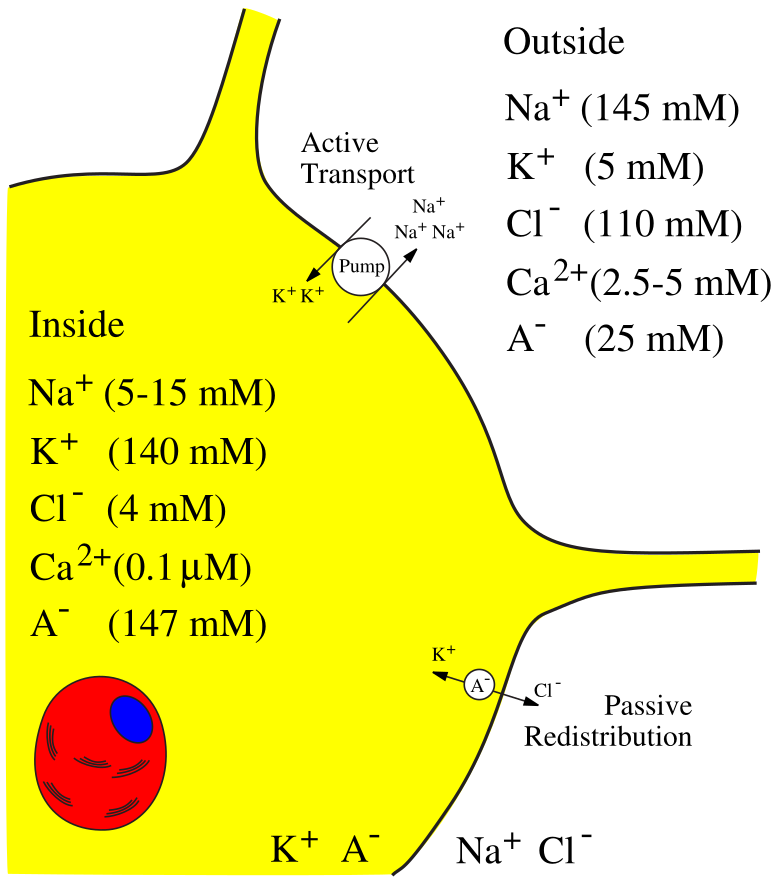
\includegraphics[width=0.7\textwidth]{./neuron_diagram.png}
\end{center}
\end{column}
\end{columns}
\end{frame}

\begin{frame}[label={sec:orgf6c6c5b}]{Whistlestop tour of electrophysiology}
\framesubtitle{Speedy sodium}

\begin{columns}
\begin{column}{0.6\columnwidth}
\begin{itemize}
\item Sodium current activates as membrane potential increases
\item Simple model: current switches on when membrane potential exceeds a threshold
\item It's an inward current, so it brings positive ions into the cell and increases membrane potential
\item This causes positive feedback!
\end{itemize}
\end{column}

\begin{column}{0.4\columnwidth}
\begin{center}
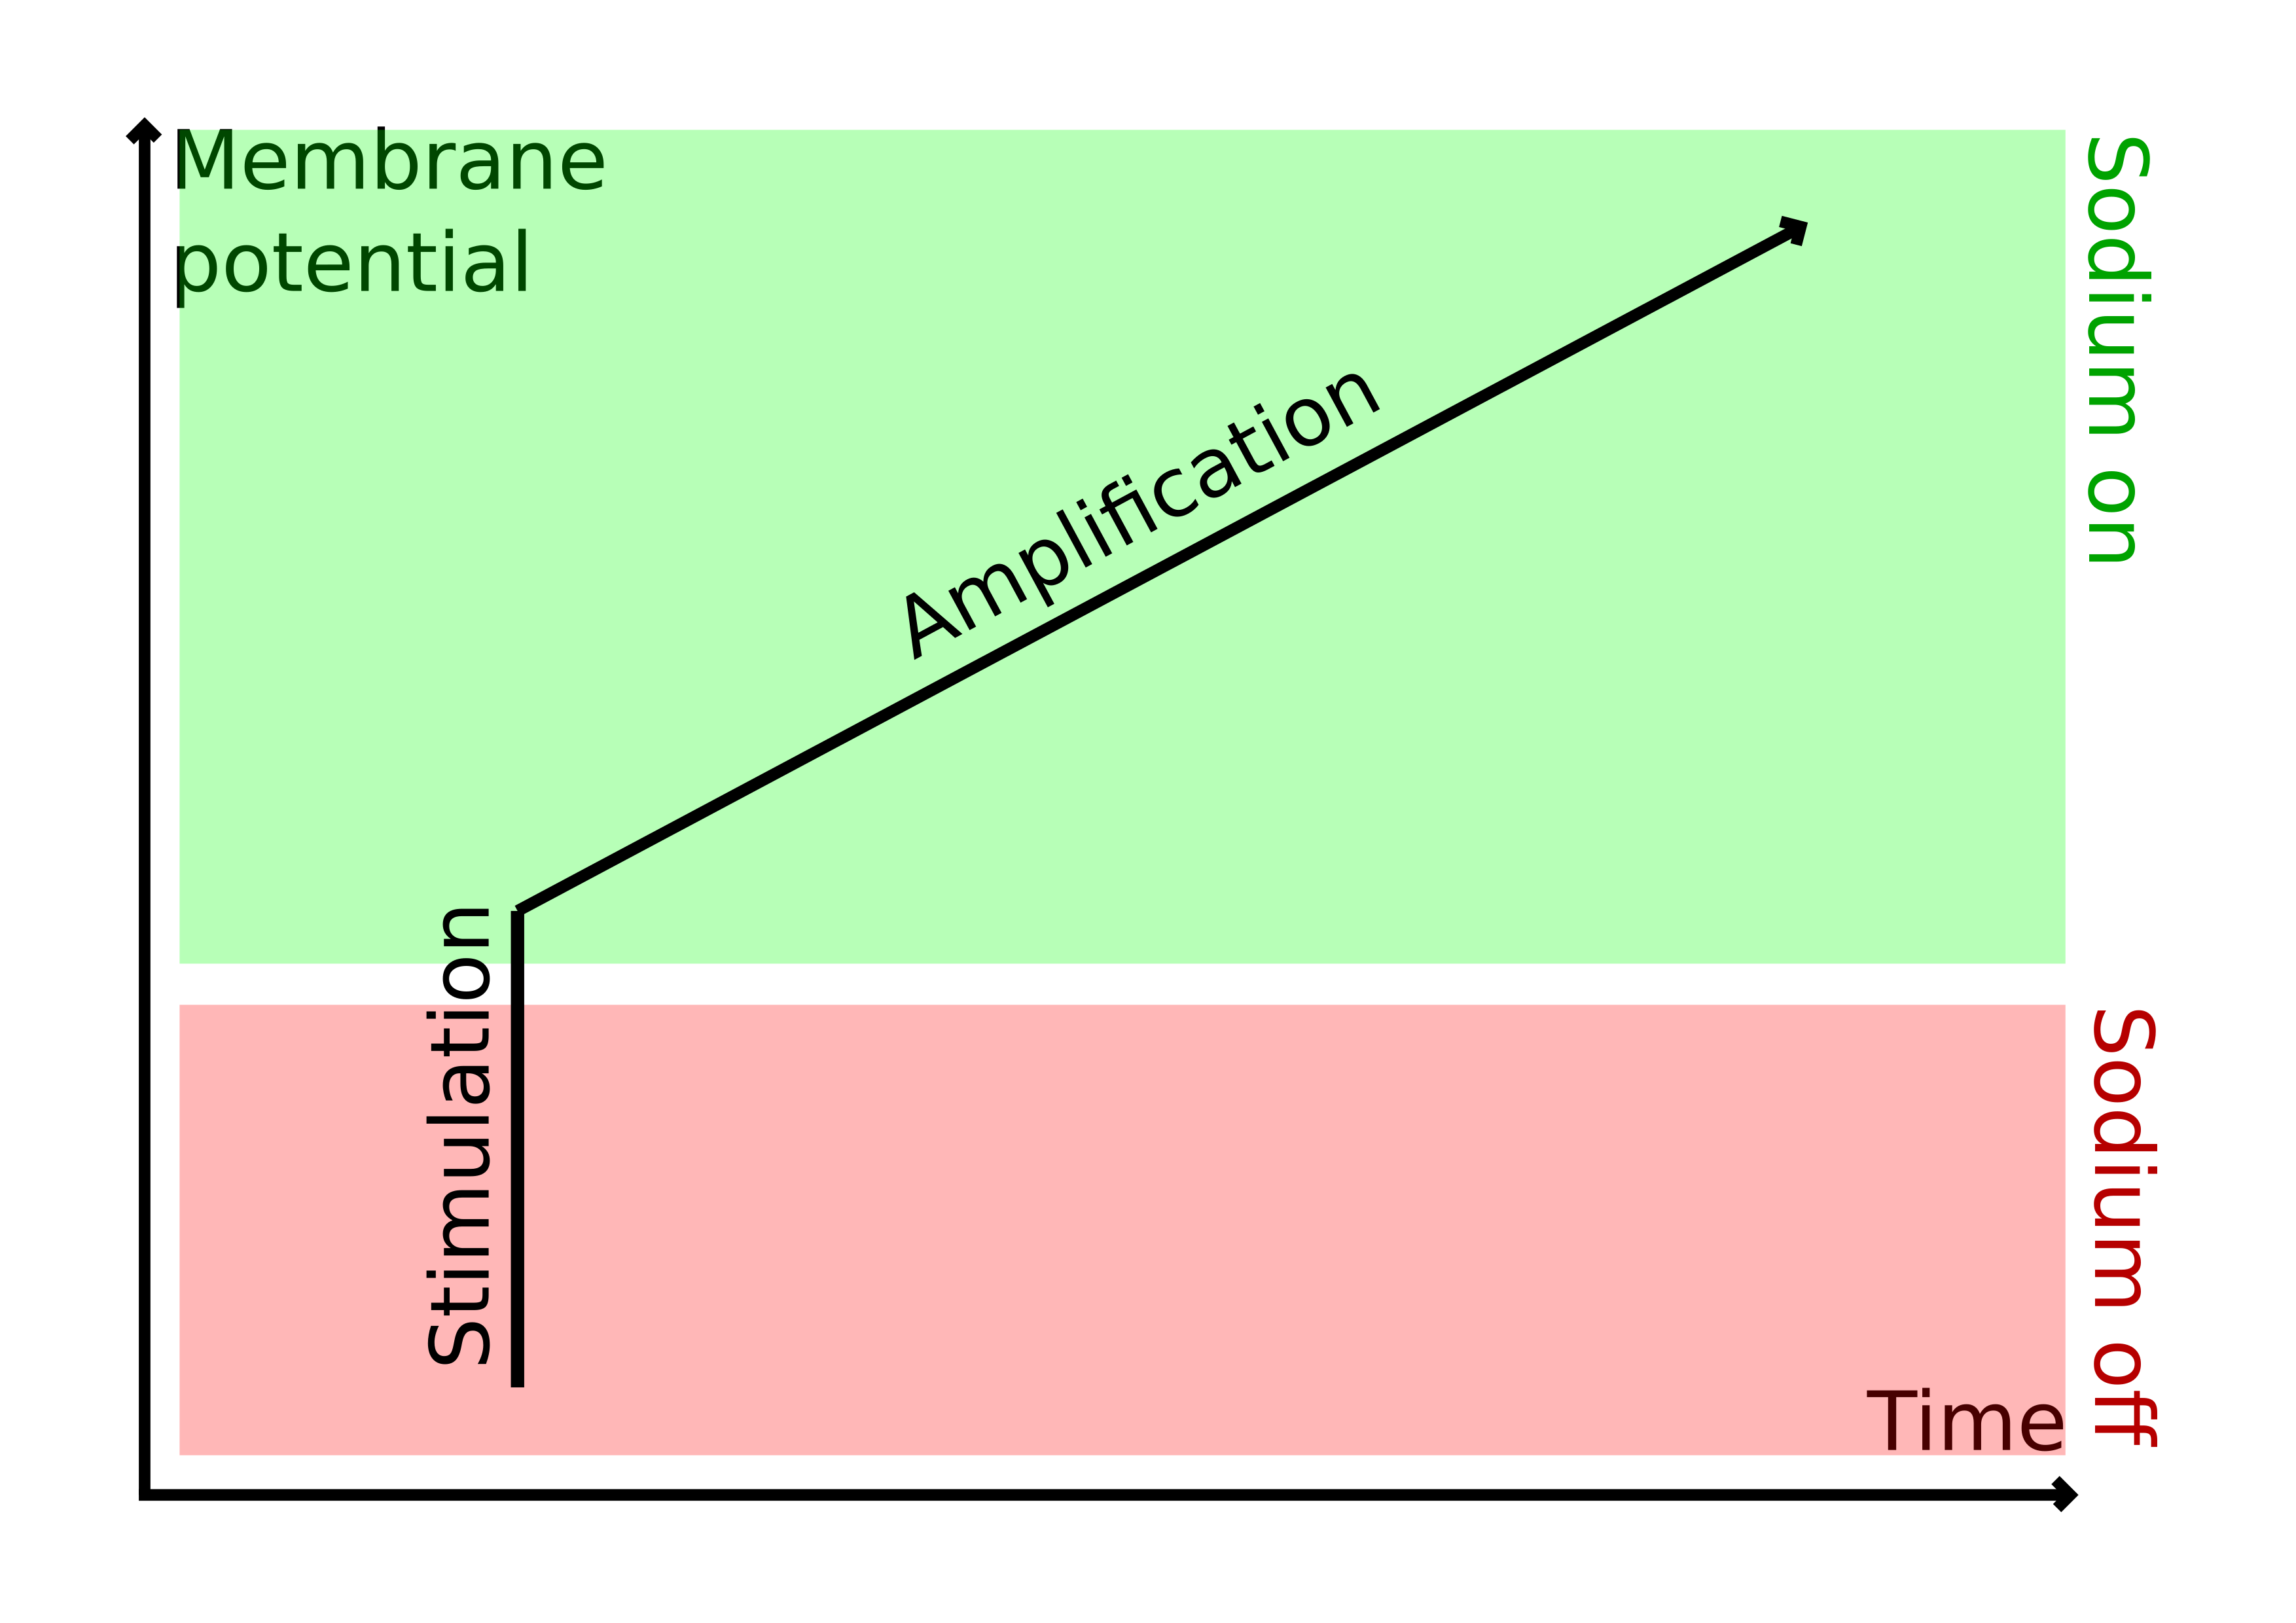
\includegraphics[width=.9\linewidth]{./fastsodium.png}
\end{center}
\end{column}
\end{columns}
\end{frame}

\begin{frame}[label={sec:org87685ef}]{Whistlestop tour of electrophysiology}
\framesubtitle{Procrastinating potassium}

\begin{columns}
\begin{column}{0.6\columnwidth}
\begin{itemize}
\item Potassium currents activate as membrane potential increases
\item Potassium forms an outward current - positive ions flow out, returning the membrane potential to its rest value
\item The potassium current turns on and off slower than the sodium current
\end{itemize}
\end{column}

\begin{column}{0.4\columnwidth}
\begin{center}
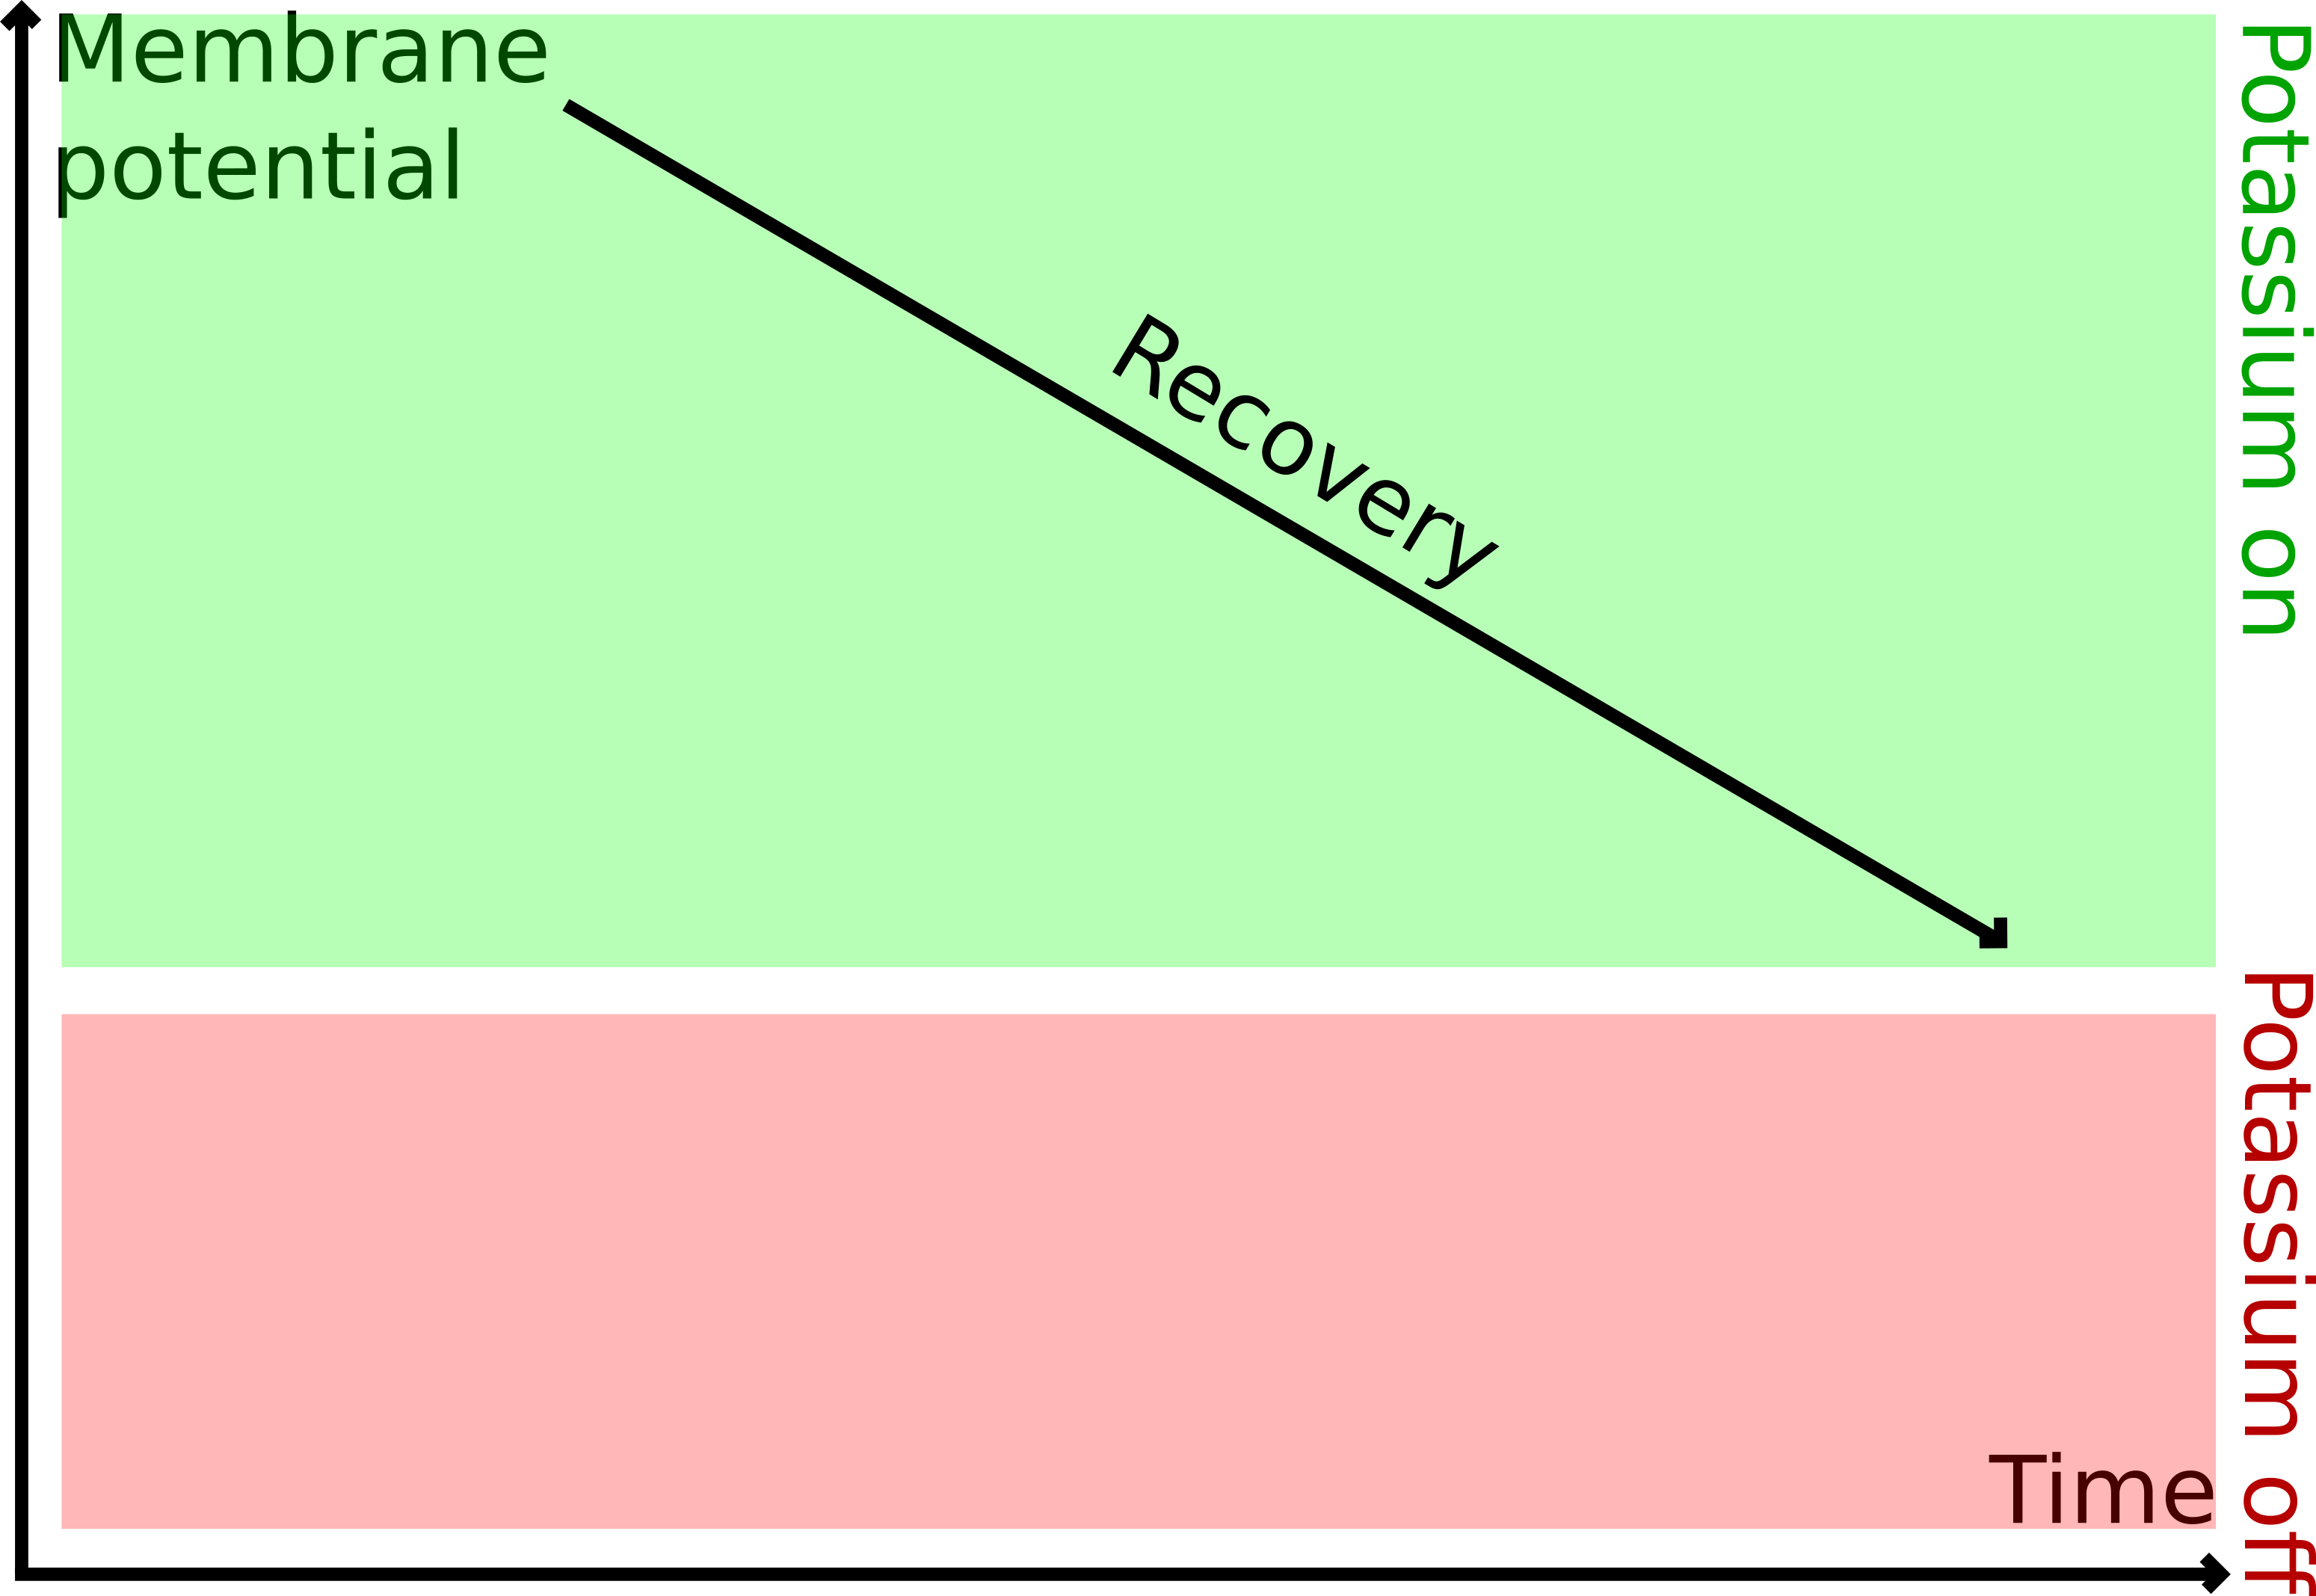
\includegraphics[width=.9\linewidth]{./slowpotassium.png}
\end{center}
\end{column}
\end{columns}
\end{frame}

\begin{frame}[label={sec:org4ca7a25}]{Whistlestop tour of electrophysiology}
\framesubtitle{Slow-fast spiking}

The interplay of slow potassium and fast sodium currents causes neurons to spike, rather than settling to a steady state

\begin{block}{A recipe for spiking}
\begin{itemize}
\item Sodium currents switch on and off fast
\item Potassium currents switch on and off slowly
\item Slow potassium activation allows the membrane potential to increase fast
\item Once it activates, the potassium current pulls the membrane potential back down
\item Potassium current takes a while to switch off again, so membrane potential gets pulled down to below the turn-on threshold for the two currents
\end{itemize}
\end{block}
\end{frame}


\begin{frame}[label={sec:org37c3372}]{Whistlestop tour of electrophysiology}
\framesubtitle{Hodgkin-Huxley formalism}

\begin{columns}
\begin{column}{0.5\columnwidth}
Currents flow through different ion channels; let's consider each one separately.
Using current laws,

\begin{equation}
    C\dot{V} = I_{Na} + I_{Ca} + I_{K} + I_{Cl}~.
\end{equation}

The Hodgkin-Huxley model gives each ionic current as a function of membrane potential.
This is exciting, as we now have a mathematical model of a neuron, to which we can apply a rigorous analysis.
\end{column}

\begin{column}{0.5\columnwidth}
\begin{center}
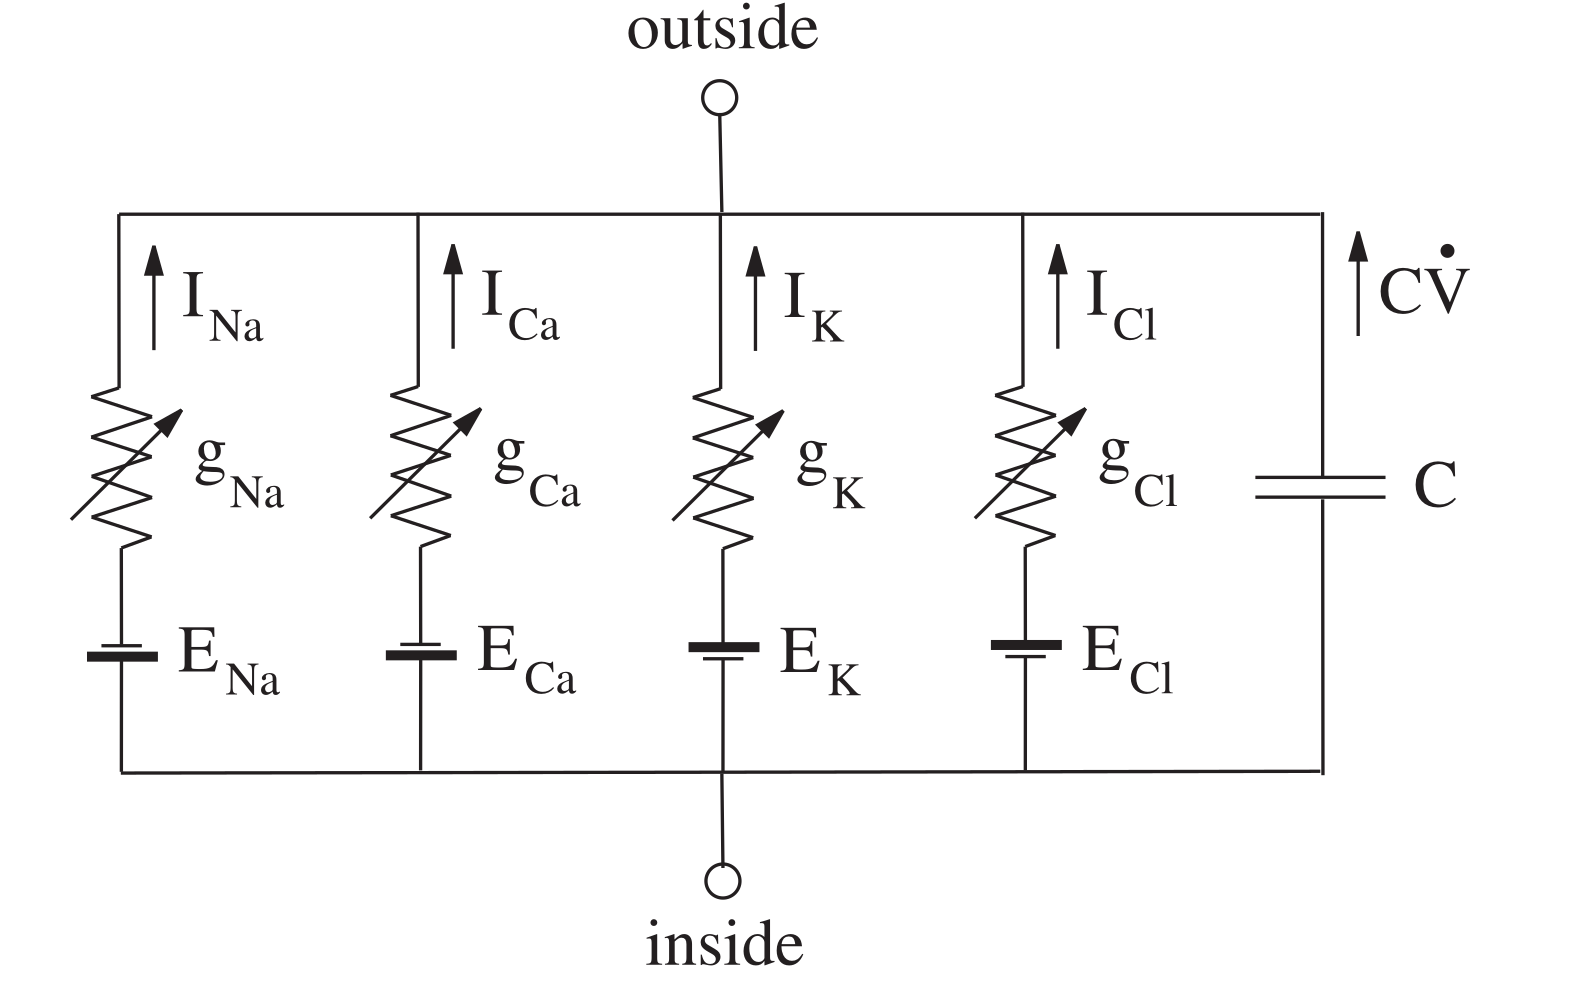
\includegraphics[width=.9\linewidth]{./neuroncircuit.png}
\end{center}
\end{column}
\end{columns}
\end{frame}

\begin{frame}[label={sec:org31c302e}]{Why are mathematicians interested in neurons?}
Neurons exhibit a wide range of complex dynamics.
Mathematical models of these dynamics can be easily tested on physical neurons.
Interesting features include\ldots{}
\begin{itemize}[<+->]
\item Highly nonlinear
\item High-dimensional
\item Multi-timescale dynamics
\item Stochastic behaviour
\end{itemize}
\end{frame}

\begin{frame}[label={sec:org5c33024}]{Aren't neurons a done science though?}
\begin{itemize}[<+->]
\item Biological literature typically describes neurons in terms of ionic currents
\item This leads to incorrect descriptions (eg. all-or-nothing spikes, thresholds)
\item A mathematical is useful because it let's us explain neural dynamics in a more rigorous, systematic way
\item Many behaviours that seem confusing when explained as ionic currents, have a very natural interpretation in dynamical systems theory
\item Dynamical neuroscience is also something of a new field, though, so there's still a big research gap in experimental bifurcation analysis
\end{itemize}
\end{frame}

\begin{frame}[label={sec:org6be62d05}]{Project goal}
Goal: develop a method of observing bifurcations in the dynamics of living neurons.
\end{frame}

\begin{frame}[plain,label={sec:org0bea7ed}]{Spike trains and neural computation}
\begin{center}
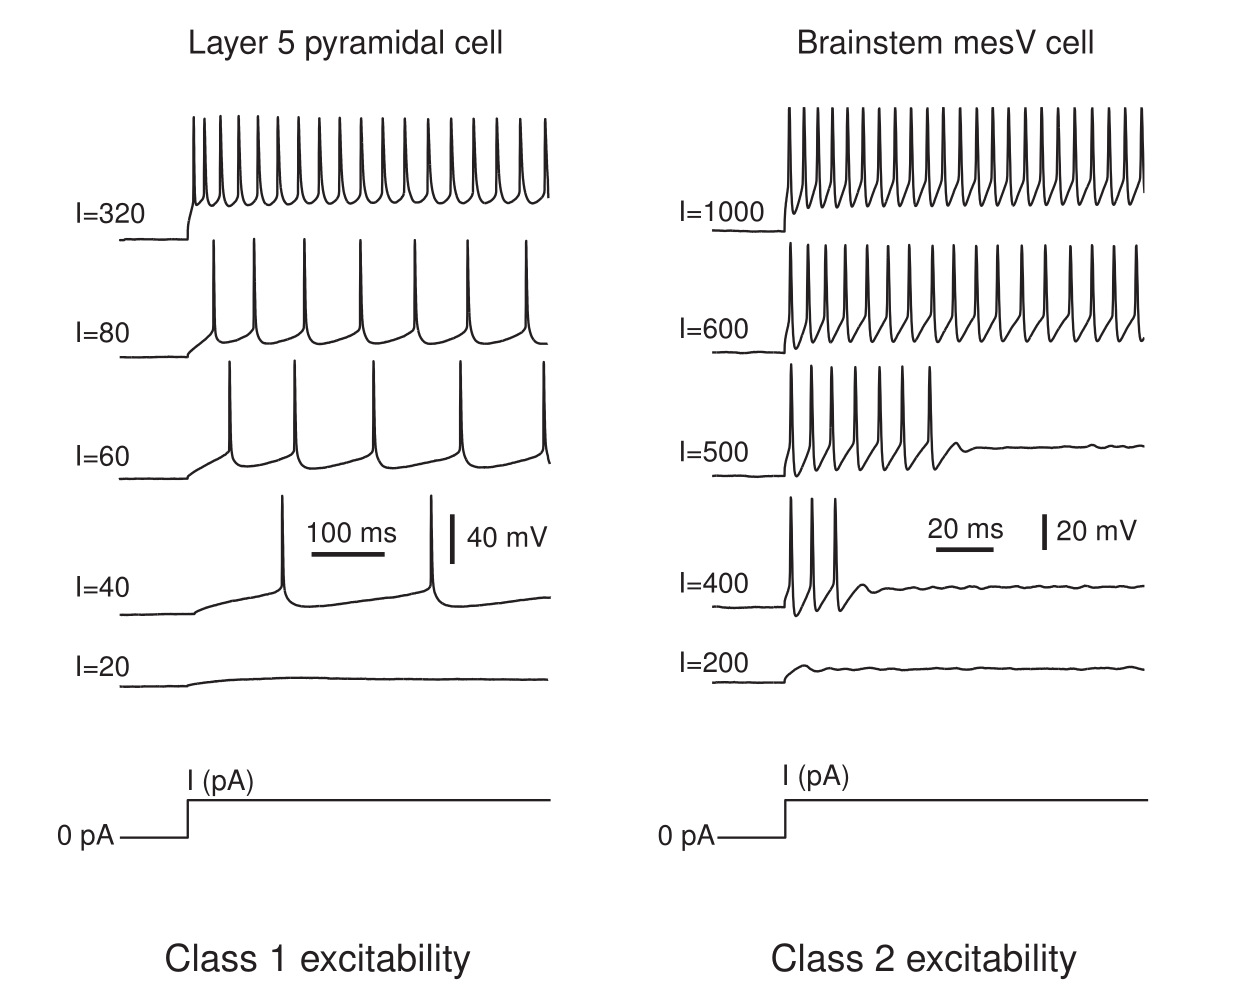
\includegraphics[height=\textheight]{./excitability_classes.png}
\end{center}
\end{frame}

\begin{frame}[plain,label={sec:org0951dc1}]{Phase diagrams}
\begin{center}
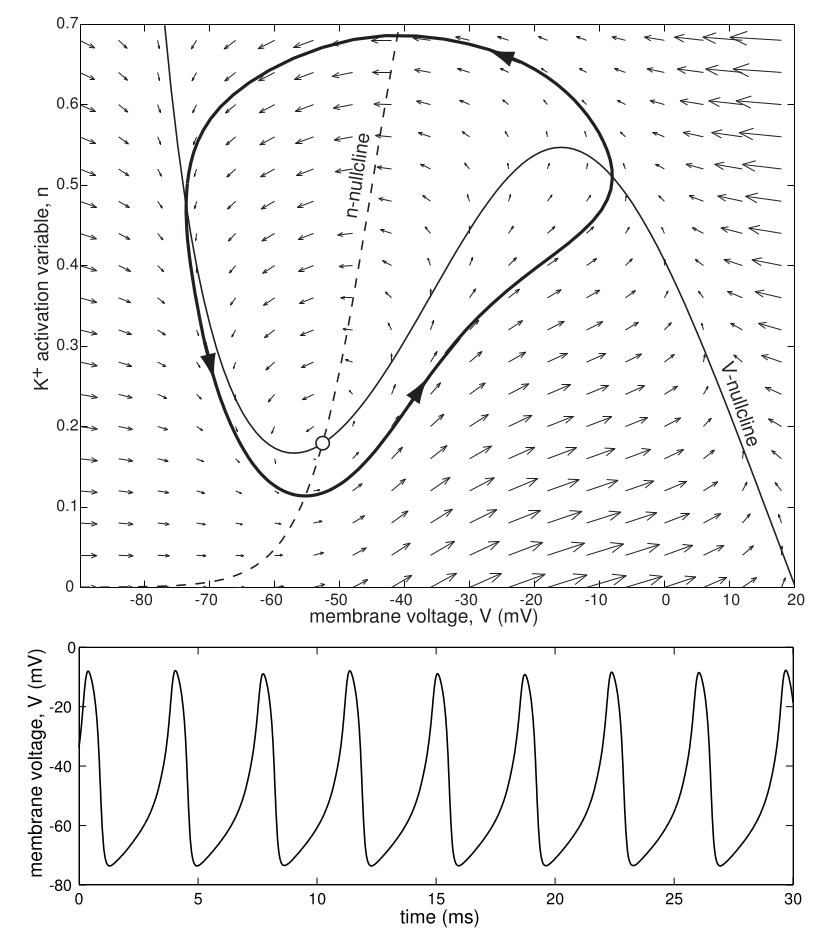
\includegraphics[height=\textheight]{./phaseplane.png}
\end{center}
\end{frame}

\begin{frame}[label={sec:org0651f9c}]{Bifurcations}
\begin{center}
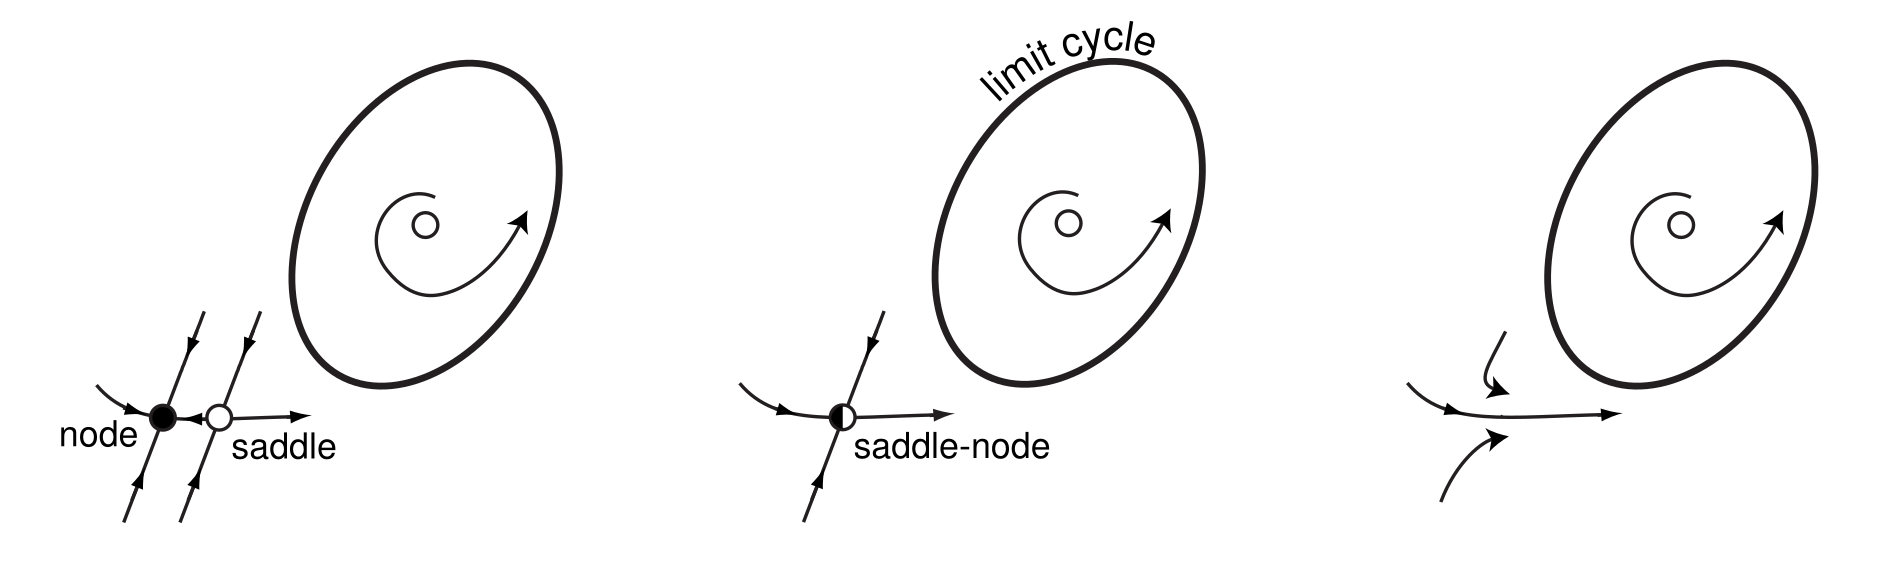
\includegraphics[width=.9\linewidth]{./saddlenode.png}
\end{center}
\end{frame}

\begin{frame}[label={sec:org56d9c8d}]{Bifurcations}
\begin{center}
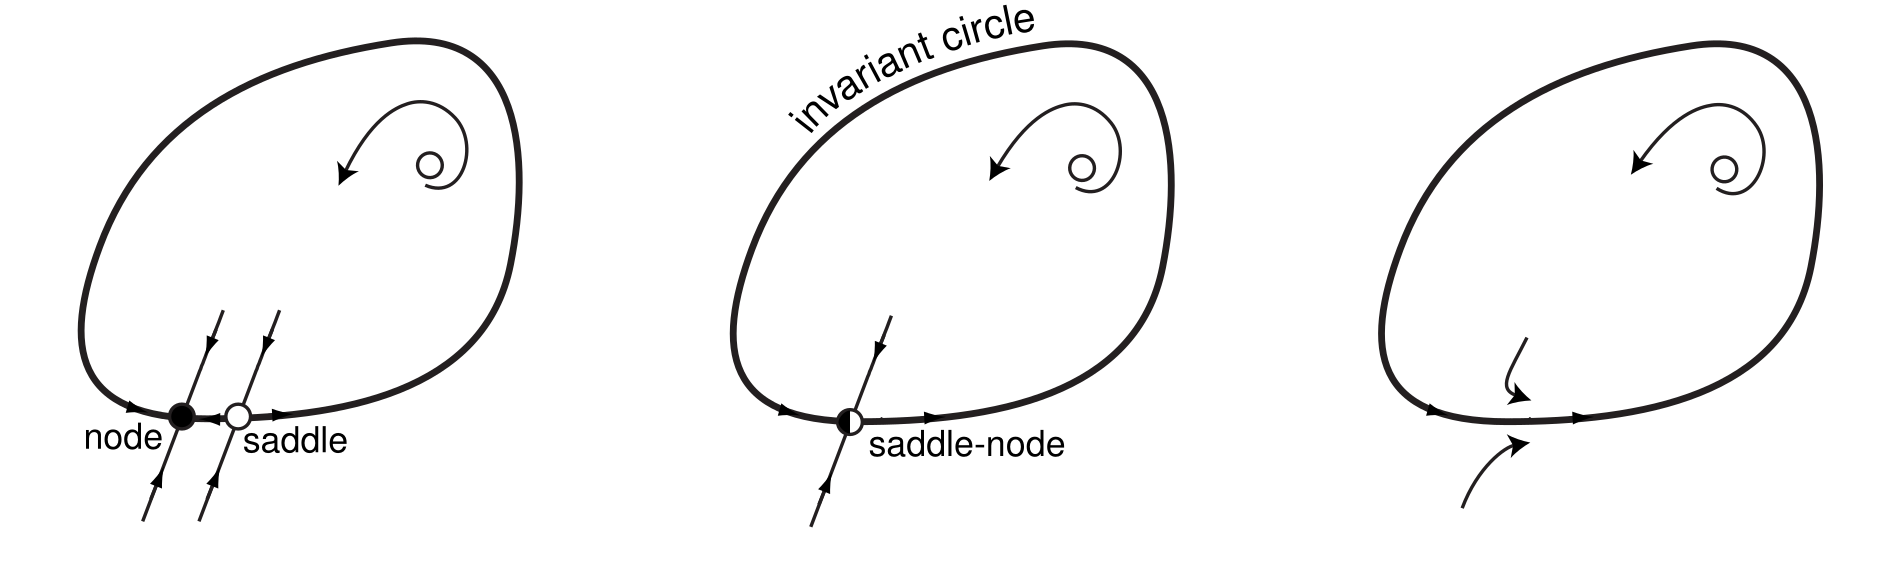
\includegraphics[width=.9\linewidth]{./snic.png}
\end{center}
\end{frame}

\begin{frame}[label={sec:orgdf3da99}]{Bifurcations}
\begin{center}
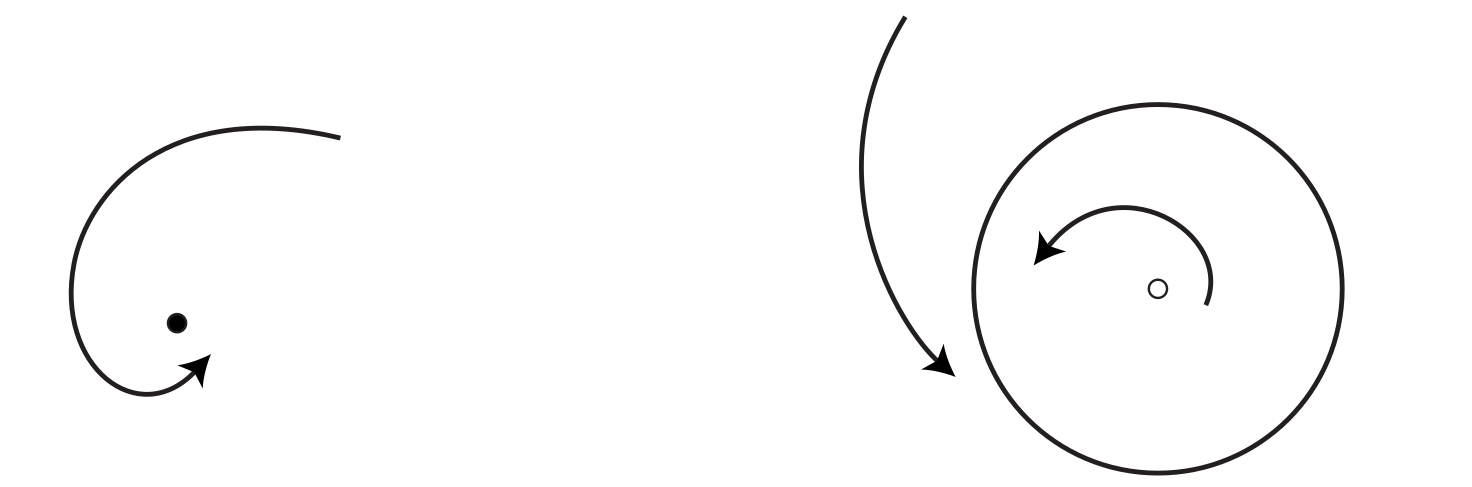
\includegraphics[width=.9\linewidth]{./hopf1.png}
\end{center}
\end{frame}

\begin{frame}[label={sec:orgf820b55}]{Bifurcations}
\begin{center}
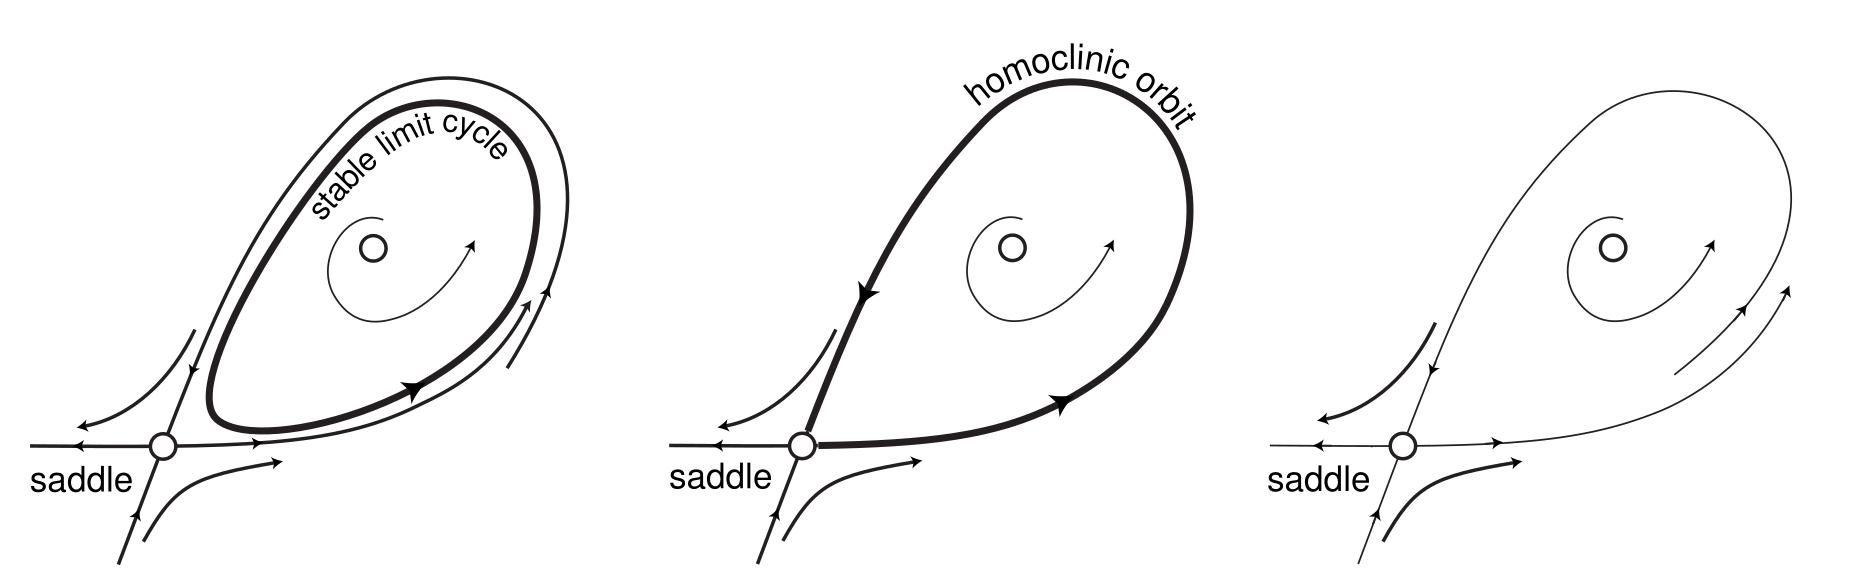
\includegraphics[width=.9\linewidth]{./homoclinic.png}
\end{center}
\end{frame}


\begin{frame}[label={sec:org6be62d5}]{Project goal}
Goal: develop a method of observing bifurcations in the dynamics of living neurons.


\vspace{1cm}
\begin{block}{George Box}
All models are wrong, but some are useful
\end{block}
\end{frame}



\begin{frame}[label={sec:org44e7ad1}]{Numerical continuation}
Consider \(f(x,\lambda)=0\).
Numerical continuation seeks to track \(x\), as \(\lambda\) varies.
For ODEs of form

$$\dot{x} = f(x,\lambda)~~,$$

this can be used to find bifurcations.
\end{frame}

\begin{frame}[label={sec:org948d6a3}]{Numerical continuation}
\begin{center}
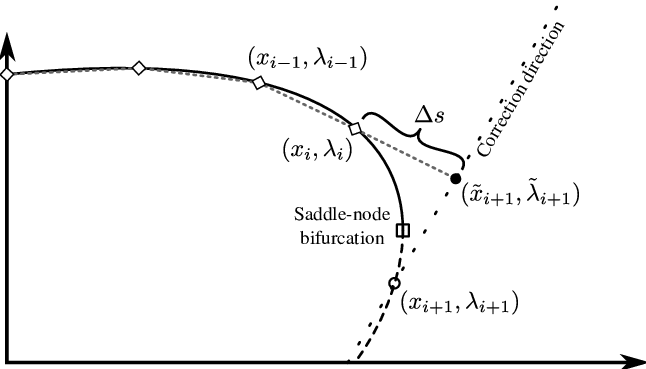
\includegraphics[height=0.8\textheight]{./continuation.png}
\end{center}
\end{frame}

\begin{frame}[label={sec:orgd6fd462}]{Control-based continuation}
CBC allows us to apply continuation methods on black-box numerical or physical systems, no model needed.

\begin{itemize}
\item Use control theory to steer the system onto a (possibly unstable) natural invariant set
\item Track that invariant set as the bifurcation parameter changes
\end{itemize}

This tracking step can be a classical psuedo-arclength continuation, or something more problem-specific.
\end{frame}


\begin{frame}[label={sec:orgcf4b8b7}]{Research problems}
\begin{itemize}[<+->]
\item How do we control a highly nonlinear black-box system?
\item How can CBC be extended to study global bifurcations?
\item How do we efficiently discretise spiking signals?
\item Neurons are inherently stochastic; how do we deal with controlling and analysing this?
\item The system has poor observability (eg. can't easily see population ion channel conductance); how do we control a system that we can't observe?
\item We have limited control inputs; how can we use them to steer the dynamics effectively?
\end{itemize}
\end{frame}
\end{document}
